% =====================================================================
%  CAPÍTULO 5 · IMPLEMENTACIÓN
%  Función: contar cómo se ha construido la solución y conectar cada parte
%  con los requisitos. Que se vea el trabajo real.
%  Reglas clave:
%   - Organiza por componentes, no por orden cronológico.
%   - Estructura del código y cómo se conectan los componentes.
%   - Fragmentos de código SOLO si aportan (10-25 líneas) y siempre
%     explicados; el código completo va en el repositorio (Apéndice A).
%   - En una app: capturas REALES de la aplicación, agrupadas (2-3 por
%     figura), y legibles.
%   - Explica errores, seguridad y privacidad donde apliquen.
%   - Definiciones técnicas exactas (p. ej. qué se cifra y con qué).
% =====================================================================
\chapter{Implementación}
\label{cap:implementacion}

Este capítulo describe cómo se han implementado los componentes de la
arquitectura presentada en la Sección~\ref{sec:arquitectura}.

\section{Estructura del código}
\label{sec:estructura-codigo}

El código se organiza en dos módulos dentro del mismo repositorio
(Apéndice~\ref{ap:repositorio}): \texttt{app/}, con la aplicación Android, y
\texttt{servidor/}, con la \ac{API} y el acceso a datos. El
Listado~\ref{lst:estructura} muestra las carpetas principales del servidor.

\begin{lstlisting}[float, language={}, numbers=none, caption={Estructura de carpetas del servidor.},
                   label={lst:estructura}]
servidor/
|-- api/          rutas de la API (salas, reservas, usuarios)
|-- dominio/      reglas de negocio (p. ej. solapamiento de reservas)
|-- datos/        acceso a la base de datos
`-- pruebas/      pruebas unitarias y de integración
\end{lstlisting}

\section{Gestión de reservas}
\label{sec:gestion-reservas}

La regla que impide reservas solapadas (RF-04) es la parte más delicada del
sistema, porque dos usuarios pueden intentar reservar la misma sala a la vez. El
Listado~\ref{lst:reserva} muestra cómo se resuelve: la comprobación y la
inserción se ejecutan dentro de una misma transacción (línea 4), de modo que la
segunda petición ve la reserva de la primera y recibe un error 409 (línea 10) en
lugar de crear un duplicado.

% [float]: el listado se coloca entero donde quepa, sin partirse entre páginas.
\begin{lstlisting}[float, language=Python, caption={Creación de una reserva sin solapamientos.},
                   label={lst:reserva}]
@router.post("/reservas", status_code=201)
def crear_reserva(datos: ReservaIn, db: Session = Depends(get_db)):
    """Crea una reserva si la sala está libre en esa franja (RF-04)."""
    with db.begin():                       # una única transacción
        solapada = db.query(Reserva).filter(
            Reserva.sala_id == datos.sala_id,
            Reserva.inicio < datos.fin, Reserva.fin > datos.inicio,
        ).with_for_update().first()
        if solapada:
            raise HTTPException(409, "La sala ya está reservada")
        reserva = Reserva(**datos.dict())
        db.add(reserva)
    return reserva
\end{lstlisting}

\section{Aplicación móvil}
\label{sec:app}

La Figura~\ref{fig:capturas} muestra dos pantallas reales de la aplicación. En
la pantalla de inicio (Figura~\ref{fig:captura-inicio}) el usuario ve qué salas
están libres en ese momento (RF-01); al pulsar una sala libre pasa directamente
al formulario de reserva (Figura~\ref{fig:captura-reserva}), que solo pide la
franja y el número de asistentes, de modo que la reserva se completa en dos
pasos (RF-02).

\begin{figure}[htbp]
  \centering
  \begin{subfigure}[b]{0.32\textwidth}
    \centering
    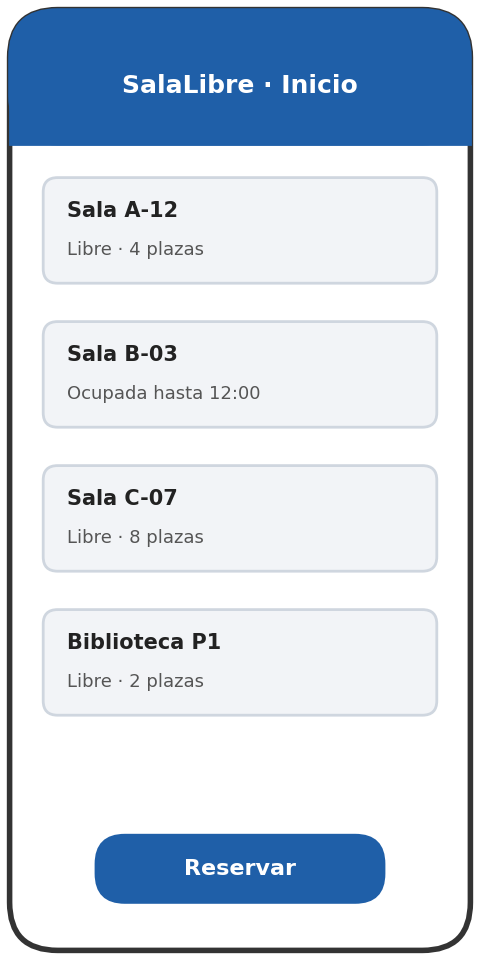
\includegraphics[width=\linewidth]{captura_inicio}
    \caption{Pantalla de inicio.}
    \label{fig:captura-inicio}
  \end{subfigure}\hspace{1.5cm}%
  \begin{subfigure}[b]{0.32\textwidth}
    \centering
    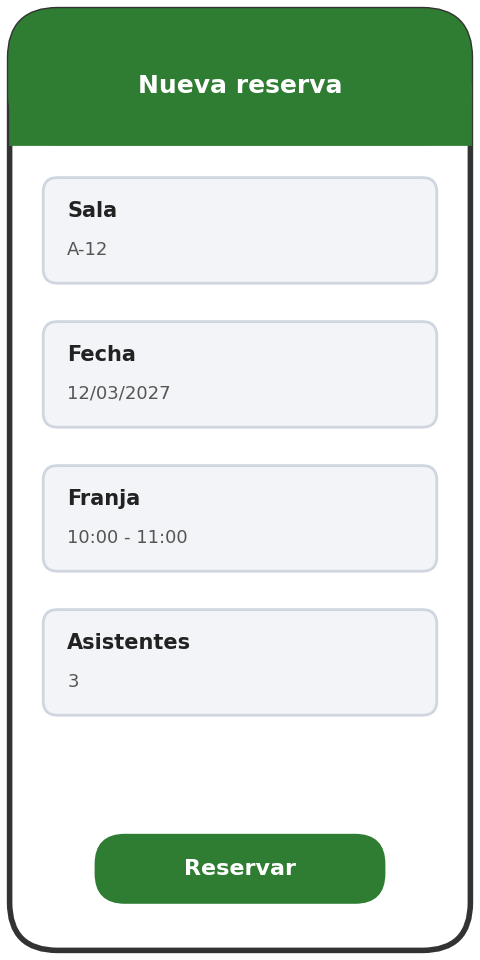
\includegraphics[width=\linewidth]{captura_reserva}
    \caption{Formulario de reserva.}
    \label{fig:captura-reserva}
  \end{subfigure}
  \caption{Pantallas principales de la aplicación.}
  \label{fig:capturas}
  \fuente{Elaboración propia (capturas de la aplicación).}
\end{figure}

% GUÍA: para una app, graba además un vídeo demo (YouTube no listado) y
% enlázalo con URL y código QR (Apéndice A). La memoria debe entenderse
% igualmente sin el vídeo.

\section{Seguridad y gestión de errores}
\label{sec:seguridad}

Explica las decisiones de seguridad con precisión técnica. Por ejemplo: las
contraseñas se guardan con una función de \emph{hash} con sal (RNF-03) y nunca
viajan en claro; las sesiones se gestionan con un \emph{token} firmado por el
servidor. Describe también qué ve el usuario cuando falla la red o una
petición, y cómo se registran los errores en el servidor.
